\subsection{Reprezentacja ruchu}
\label{subsec:reprezentacja-ruchu}

Podobnie jak przy długiej notacji szachowej, informacjami wystarczającymi do zakodowania ruchu, jest jego pole startowe, pole docelowe, oraz w niektórych przypadkach typ promocji.
Ruch szachowy jest jednak podstawową strukturą danych, na której silnik musi operować.

Z tego względu słusznym wydało się zastosowanie bardziej deskryptywnej reprezentacji, aby~obliczenia wykonywane były przy inicjalizacji zmiennej, unikając ich powielania na~późniejszym etapie wyszukiwania i oceny pozycji.
Zawarto także informacje o tym, czy ruch jest roszadą, czy może podwójnym ruchem pionka, czy może jest biciem klasycznym, bądź en-passant.
Okazało to się szczególnie przydatne przy sortowaniu ruchów.

\begin{figure}[ht]
    \centering
    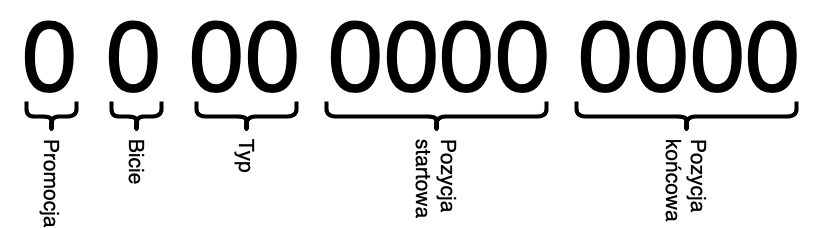
\includegraphics[width=0.85\linewidth]{rozdzialy/rozdzial01/2_reprezentacja-pozycji/rysunki/kodowanie_ruchu}
    \caption{Kodowanie ruchu szachowego}
    \label{fig:kodowanie-ruchu}
\end{figure}
